\documentclass[11pt]{article}

\usepackage[french]{babel}
\selectlanguage{french}
\usepackage[utf8]{inputenc}
\usepackage{fancyhdr}
\usepackage{lastpage}
\usepackage{listings}
\usepackage{color}
\usepackage{pdfpages}


%%%%%%%%%%
% Taille des pages (A4 serré)

\setlength{\parindent}{0pt}
\setlength{\parskip}{1ex}
\setlength{\textwidth}{17cm}
\setlength{\textheight}{24cm}
\setlength{\oddsidemargin}{-.7cm}
\setlength{\evensidemargin}{-.7cm}
\setlength{\topmargin}{-.5in}


%%%%%%%%%%
% En-têtes et pied de pages

\pagestyle{fancyplain}
\renewcommand{\headrulewidth}{0pt}
\addtolength{\headheight}{1.6pt}
\addtolength{\headheight}{2.6pt}
\lfoot{}
\cfoot{}
\rfoot{\footnotesize\sf \thepage/\pageref{LastPage}}
\lhead{\footnotesize\sf Projet GL}
\rhead{\footnotesize\sf Equipe 16} % numéro d'équipe Teide 

%%%%%%%%%%
% Informations sur le document

\title{Projet Génie Logiciel\\\emph{Charte}}

\author{BOUSSON Valentin, CONNES Cédric,\\LENTINI Sébastien, NGUY Thomas\\\emph{Equipe 16}}

\date{23 Janvier 2012}


%%%%%%%%%%
% Début du document

\begin{document}

\maketitle

\section{But de l'équipe}
Le but de l'équipe est de pouvoir rendre les livrables (maxi déca) en temps et en heure, tout en permettant l'apprentissage des méthodes de gestion d'équipe et en se respectant les uns les autres. 

\section{Compétences}
Globalement, l'équipe a un bon niveau, à la fois technique et relationnel. Si les auto-évaluations sont honnêtes, il ne devrait pas avoir de travail particulier à faire concernant une personne qui aurait des difficultés plus importantes qu'une autre, que ce soit pour la réalisation du projet ou pour la communication entre les membres.

\subsection{Compétences personelles}
Se reporter aux grilles d'auto-évaluation en annexe 1.

\subsection{Points forts et points faibles de l'équipe}

\begin{center}
  \begin{tabular}{|p{7cm}|p{7cm}|}
    \hline
    Forces & Faiblesses \\
    \hline
    \begin{itemize}
    \item Compétences techniques élevées
    \item Bonnes compétences relationnelles
    \item Habitude de travailler ensemble
    \end{itemize} 
    &
    \begin{itemize}
    \item Compétences écrite et orale
    \item Connaissances divisées en 2 groupes
    \item Connaissances techniques similaires
    \item Absence de connaissance en outils de tests
    \end{itemize}\\
    \hline
    Opportunités & Menaces \tabularnewline
    \hline
    \begin{itemize}
    \item Forte compétence en outils de debugs
    \item Facilité de communication
    \end{itemize} 
    &
    \begin{itemize}
    \item Division du groupe en sous-groupes de 2 (suivant affinités)
    \item Compétences de débug reposant sur Cédric
    \item Absence de vraie compétence sur le rédactionnel ou l'oral
    \end{itemize}\\
    \hline
  \end{tabular}
\end{center}


\section{Les valeurs communes}

Nous avons défini un ensemble de valeurs que chaque membre de l'équipe devra respecter :
\begin{itemize}
\item L'intérêt du groupe doit être privilégié par rapport aux intérêts individuels. 
\item Nous sommes exigeant dans tout ce que nous faisons.
\item Nous devons toujours respecter les opinions d'atrui, même en cas de désaccord.
\item Afin d'éviter la mauvaise ambiance au sein de l'équipe, nous nous engageons, lorsqu'un problème apparaît, à l'exprimer explicitement et à favoriser le dialogue afin de permettre sa résolution.
\item Chaque membre à le droit à l'erreur. Les autres membres devront, dans la mesure de leur possible, essayer de ne pas rejeter la faute sur quelqu'un, et essayer de surmonter les épreuves ensembles, sans laisser quelqu'un de côté.
\item Les réunions sont obligatoires.
\item Les horaires devront être respectées autant que possible, par respect envers les autres membres de l'équipe.
\item Être disponible pour le groupe, même le week end, en cas de gros problèmes dans le projet.
\item Faire confiance aux autres membres de l'équipe.
\end{itemize}

\section{Rôles et responsabilités dans l'équipe}
Hormis le chef de projet, nous n'avons pas défini de rôle particulier. Chaque membre essayera de s'approprier chaque étape du projet. En fin de projet, quand le temps ne nous le permettra plus, des rôles fixes pourront être attribués afin d'accélérer le développement.

Sébastien a été choisi comme chef d'équipe car c'était lui qui désirait le plus occuper ce poste, mais aussi car il a déjà travaillé avec Valentin et Cédric dans le passé. Son objectif consiste, avec l'aide de l'équipe, à répartir le travail entre chacun, à soutenir chaque personne dans sa tâche, à s'assurer que chacun vive son projet du mieux possible. Il a le pouvoir de décision en cas de conflit. Il animera et fera le compte rendu de chaque réunion. Il s'engage également à respecter chaque membre de l'équipe, et à concilier au mieux les souhaits de travail de chacun. Il n'a pas pour but d'exclure une personne, ou de donner des ordres. Il a ainsi un rôle de conseiller, de médiateur pour l'équipe.

\section{Préférences de travail}
\begin{itemize}
\item Le groupe travaillera ensemble à l'Ensimag, avec machine personelle (Thomas \& Valentin) ou terminal X (Sébastien \& Cédric).
\item Horaires fixe de travail de groupe : 9h-12h / 14h-17h + modulation si nécessaire
\item Réunion le matin à 9h pour définir les tâches de la journée ainsi que leur répartition.
\item Utilisation de la pause du midi pour éventuellement parler de l'avancement et des difficultés que peut rencontrer une personne dans le projet. 
\item En début de projet, essayer de varier les équipes pour renforcer la cohésion du groupe.
\end{itemize}


\newpage

\subsection*{Planning prévisionnel}
Se reporter au planning joint.

\section{Annexe}
\subsection*{Annexe 1}

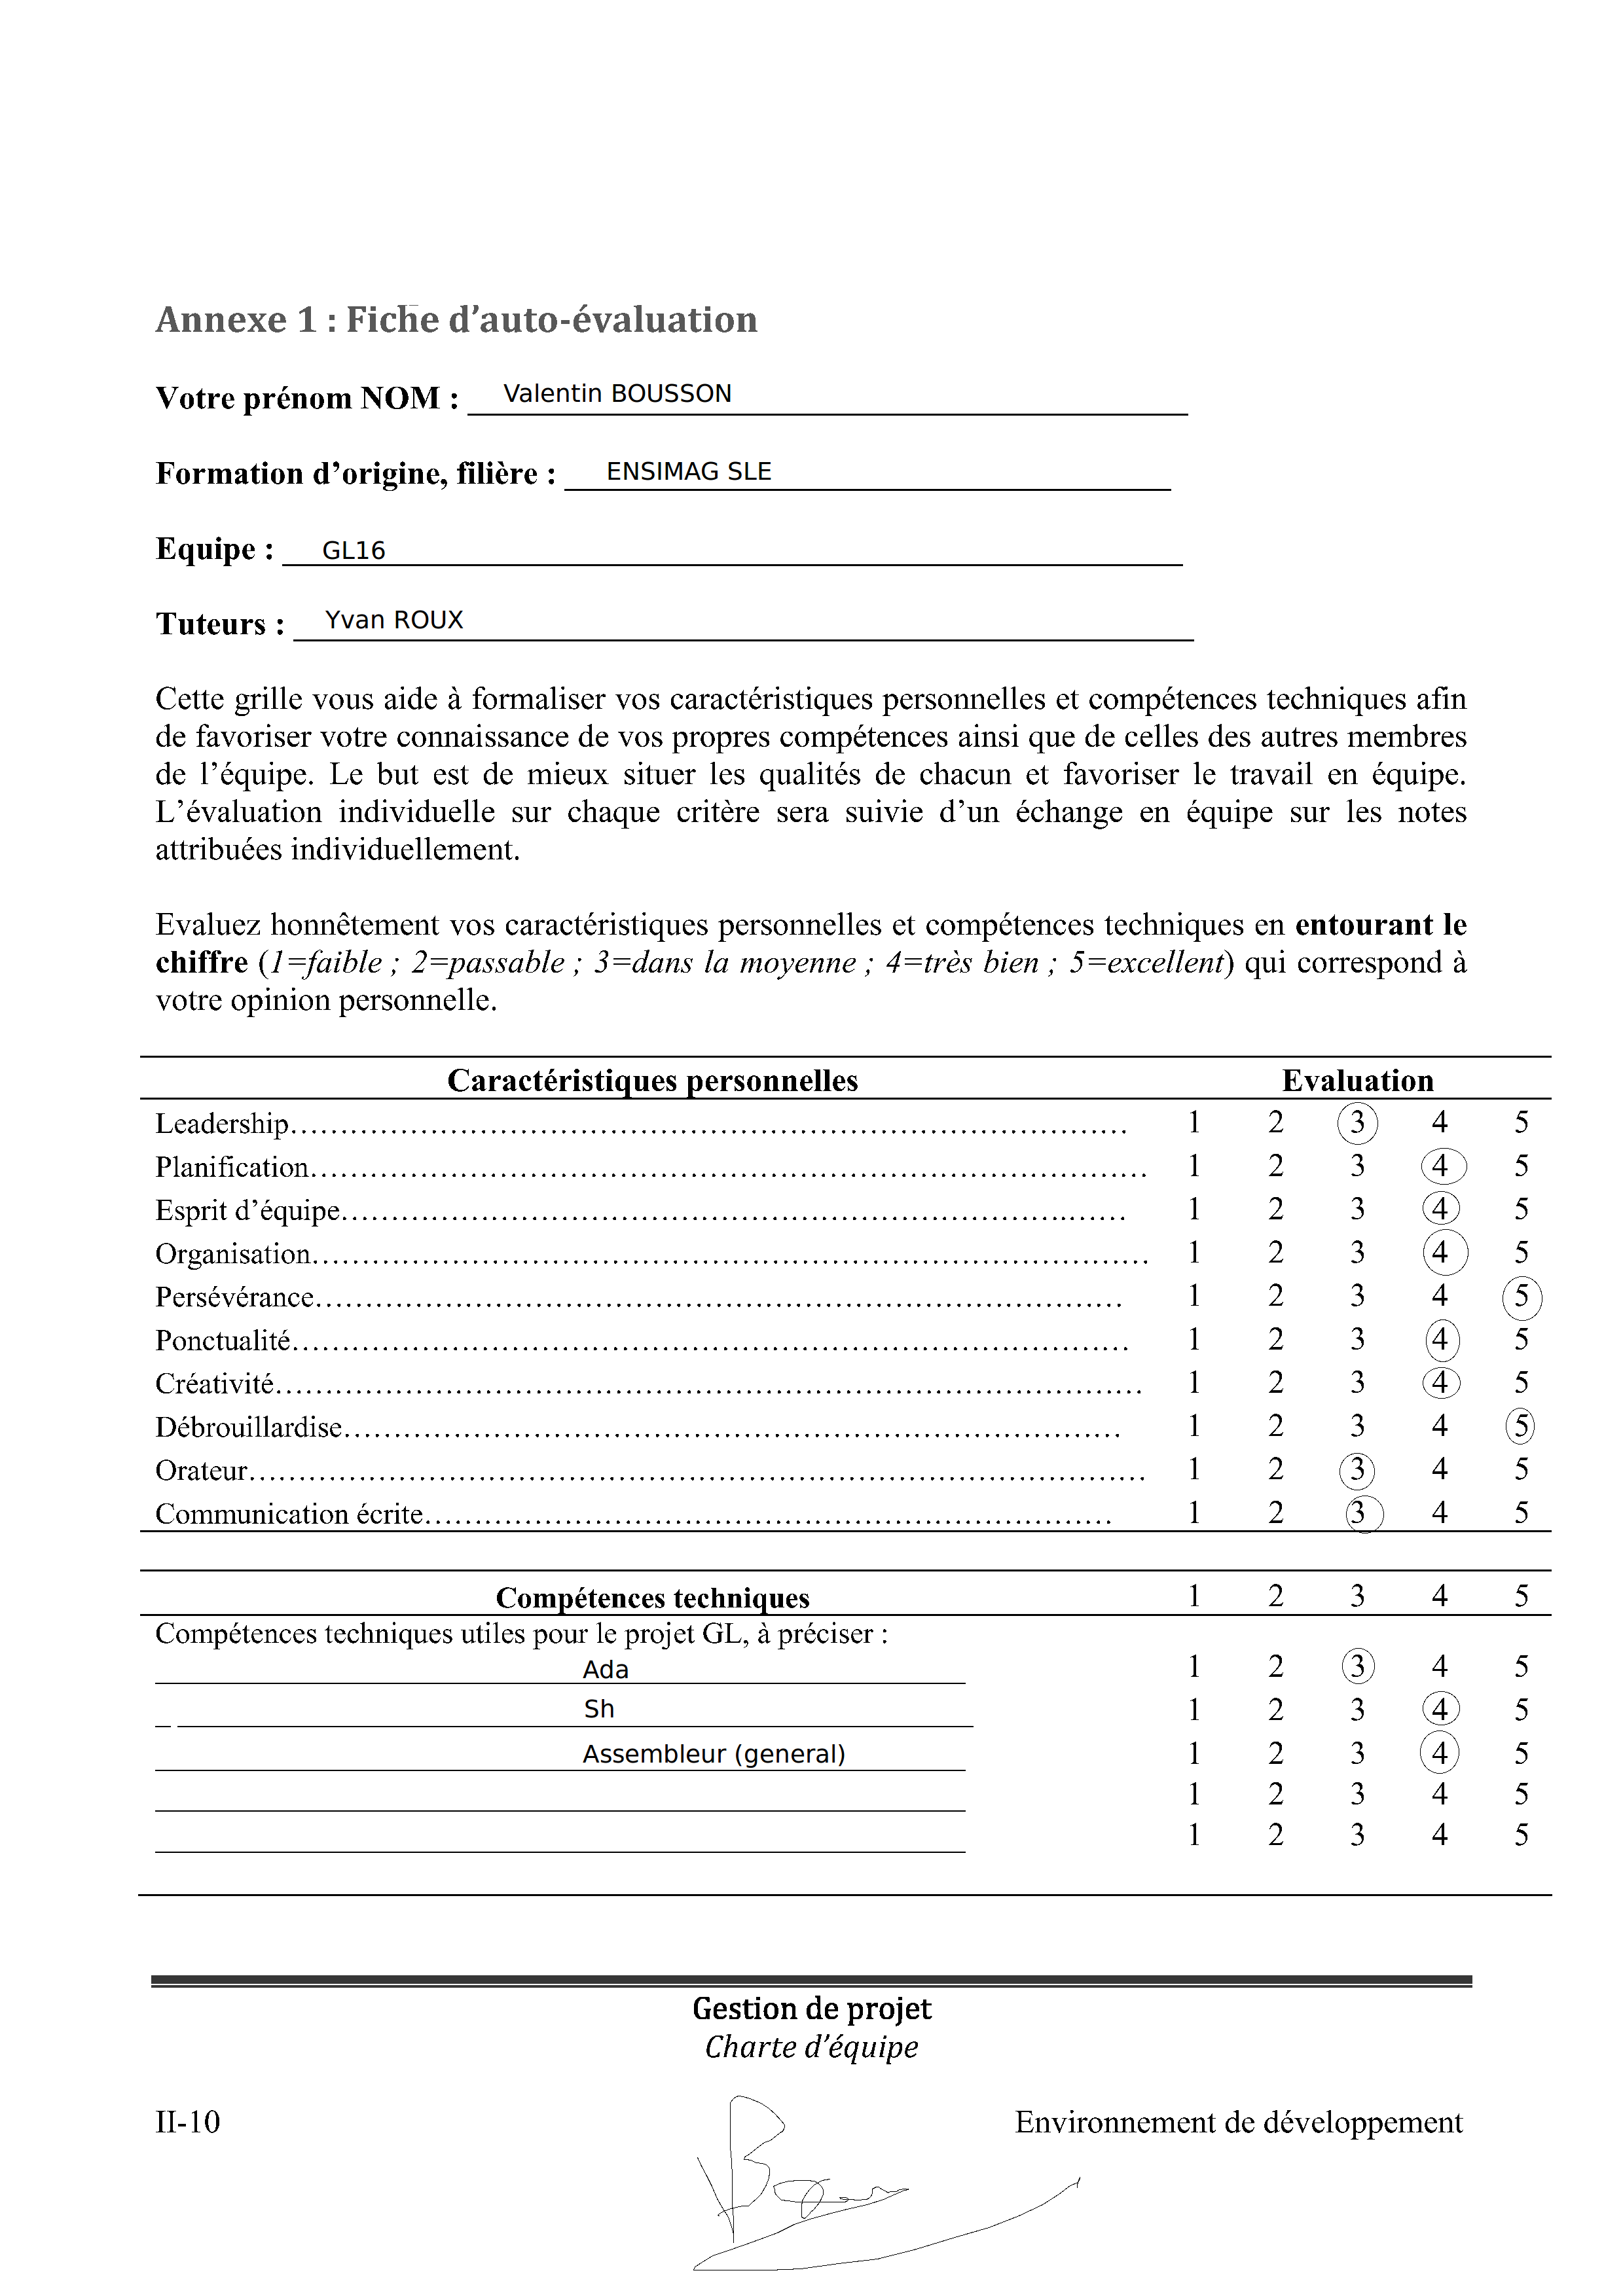
\includegraphics[scale=0.2]{auto-eval_Valentin.png}
\newpage
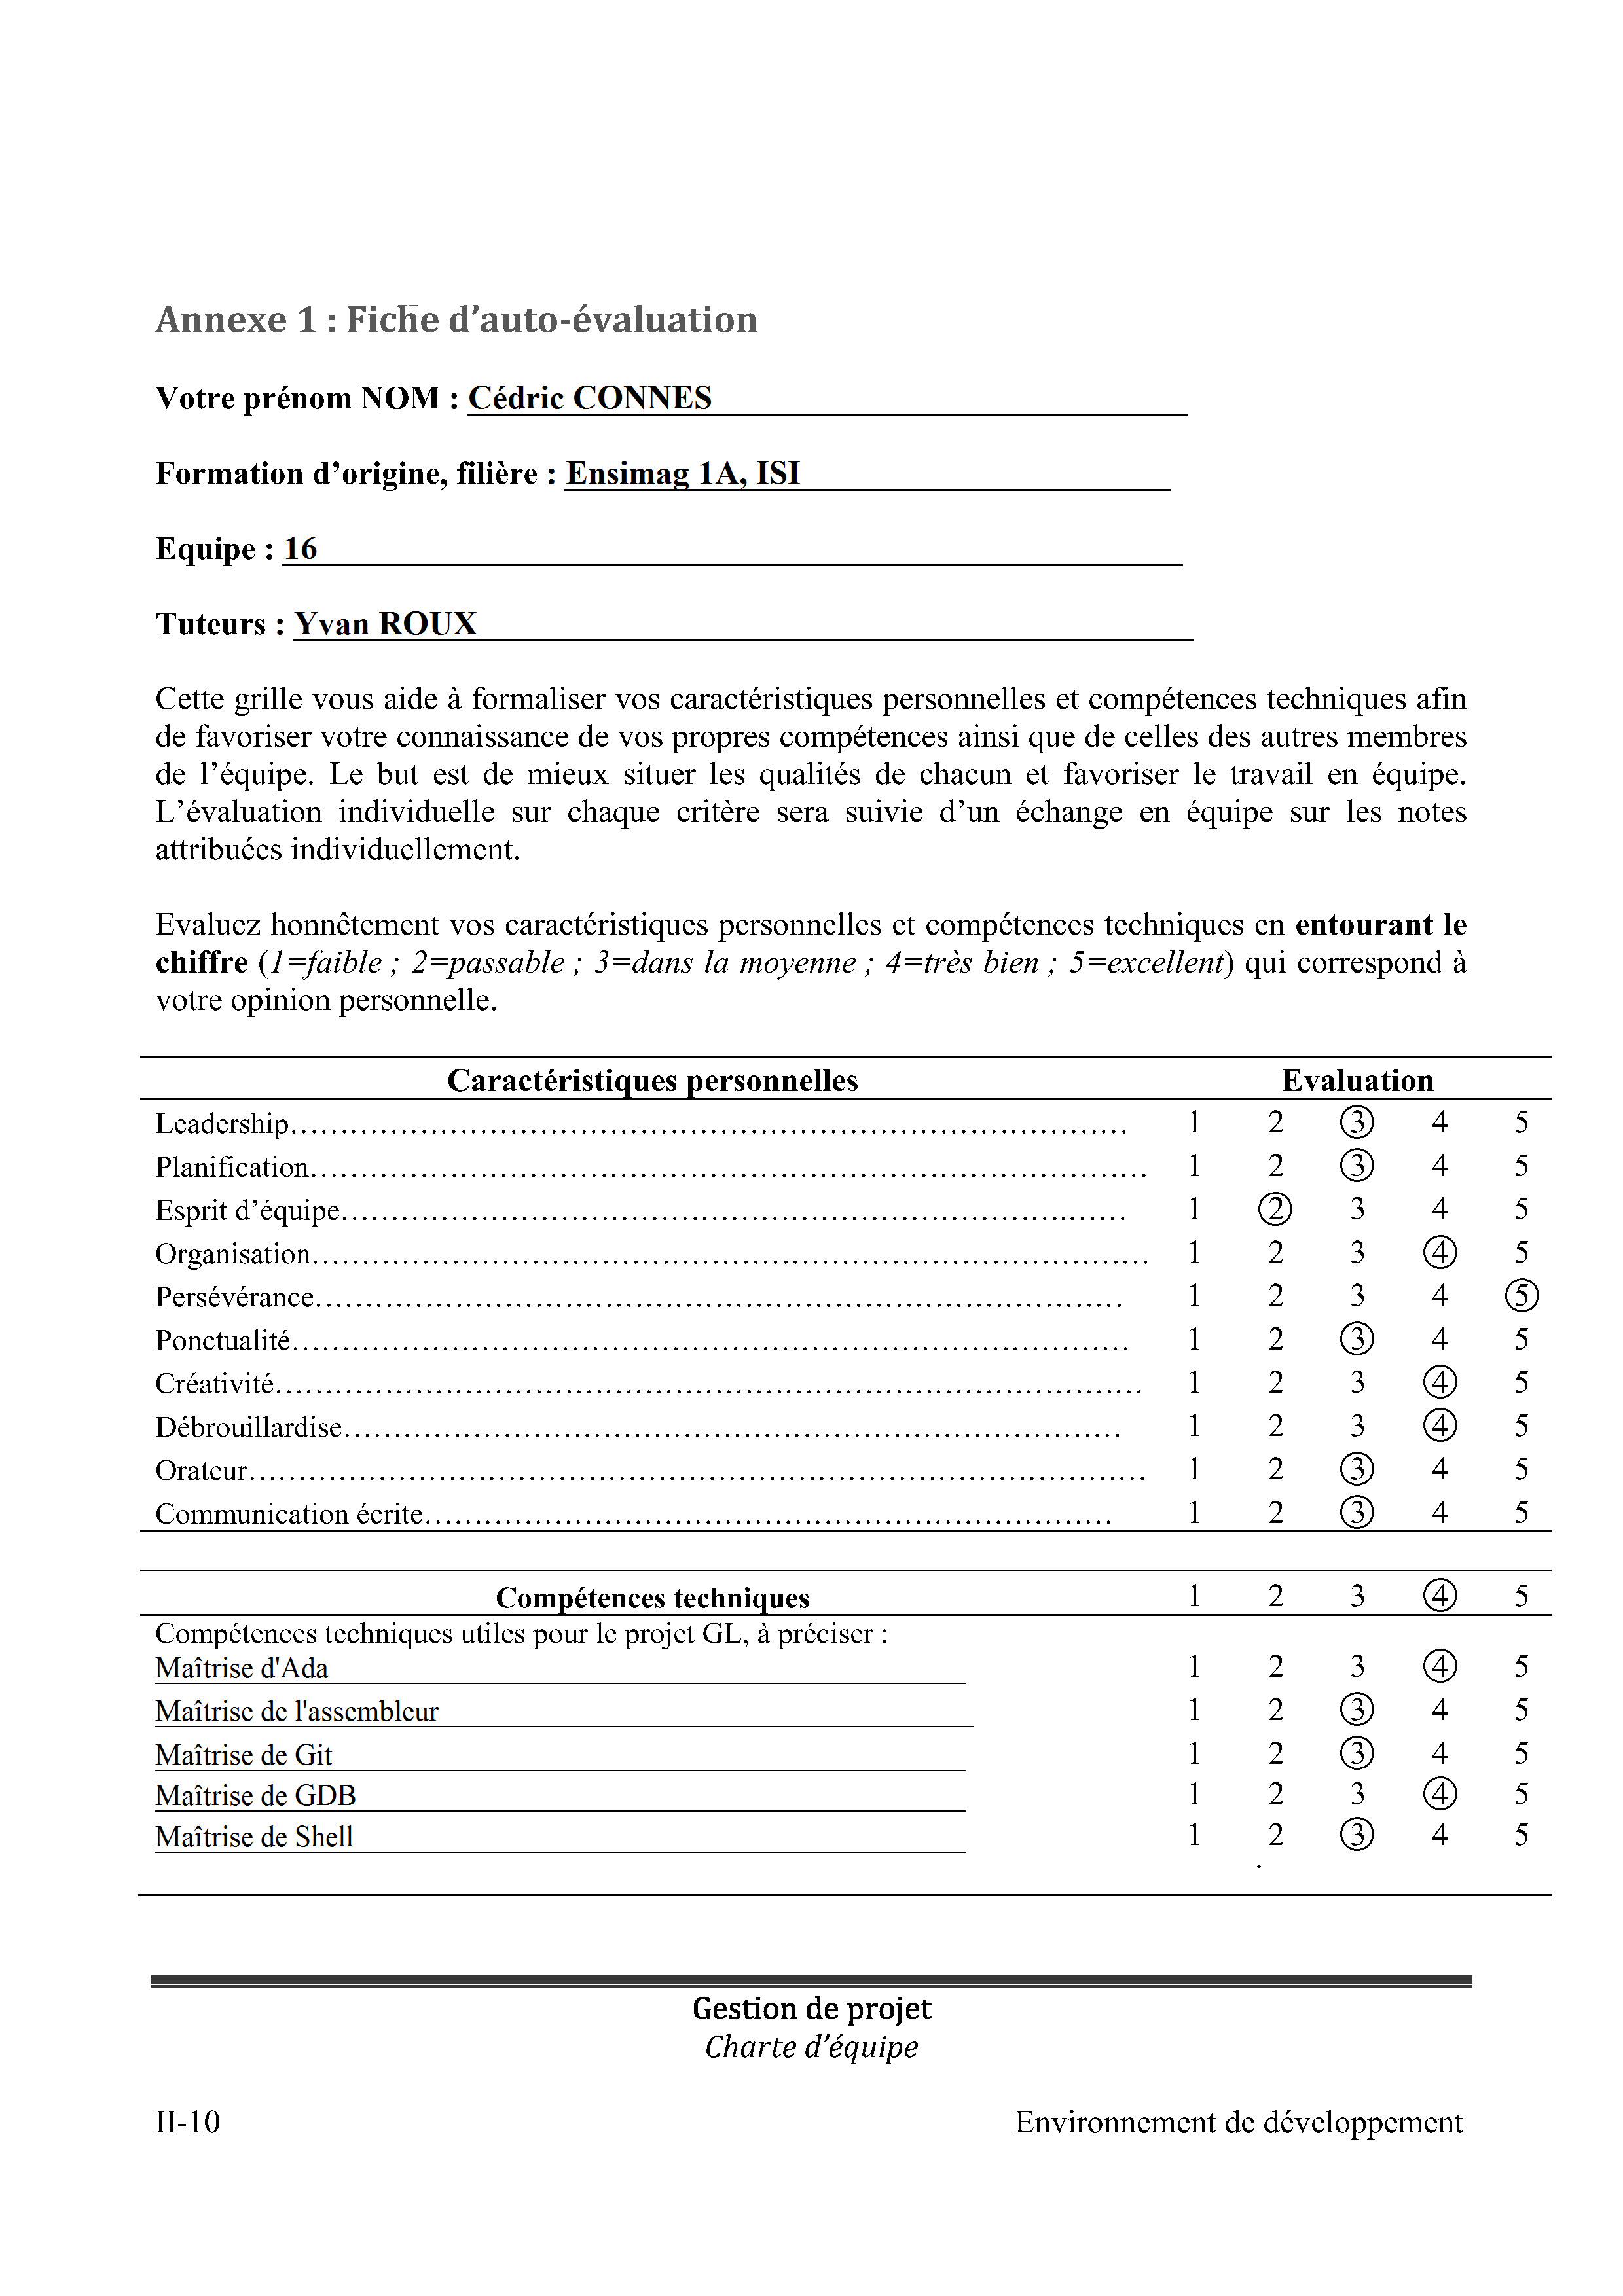
\includegraphics[scale=0.9]{auto-eval_Cedric.png}
\newpage
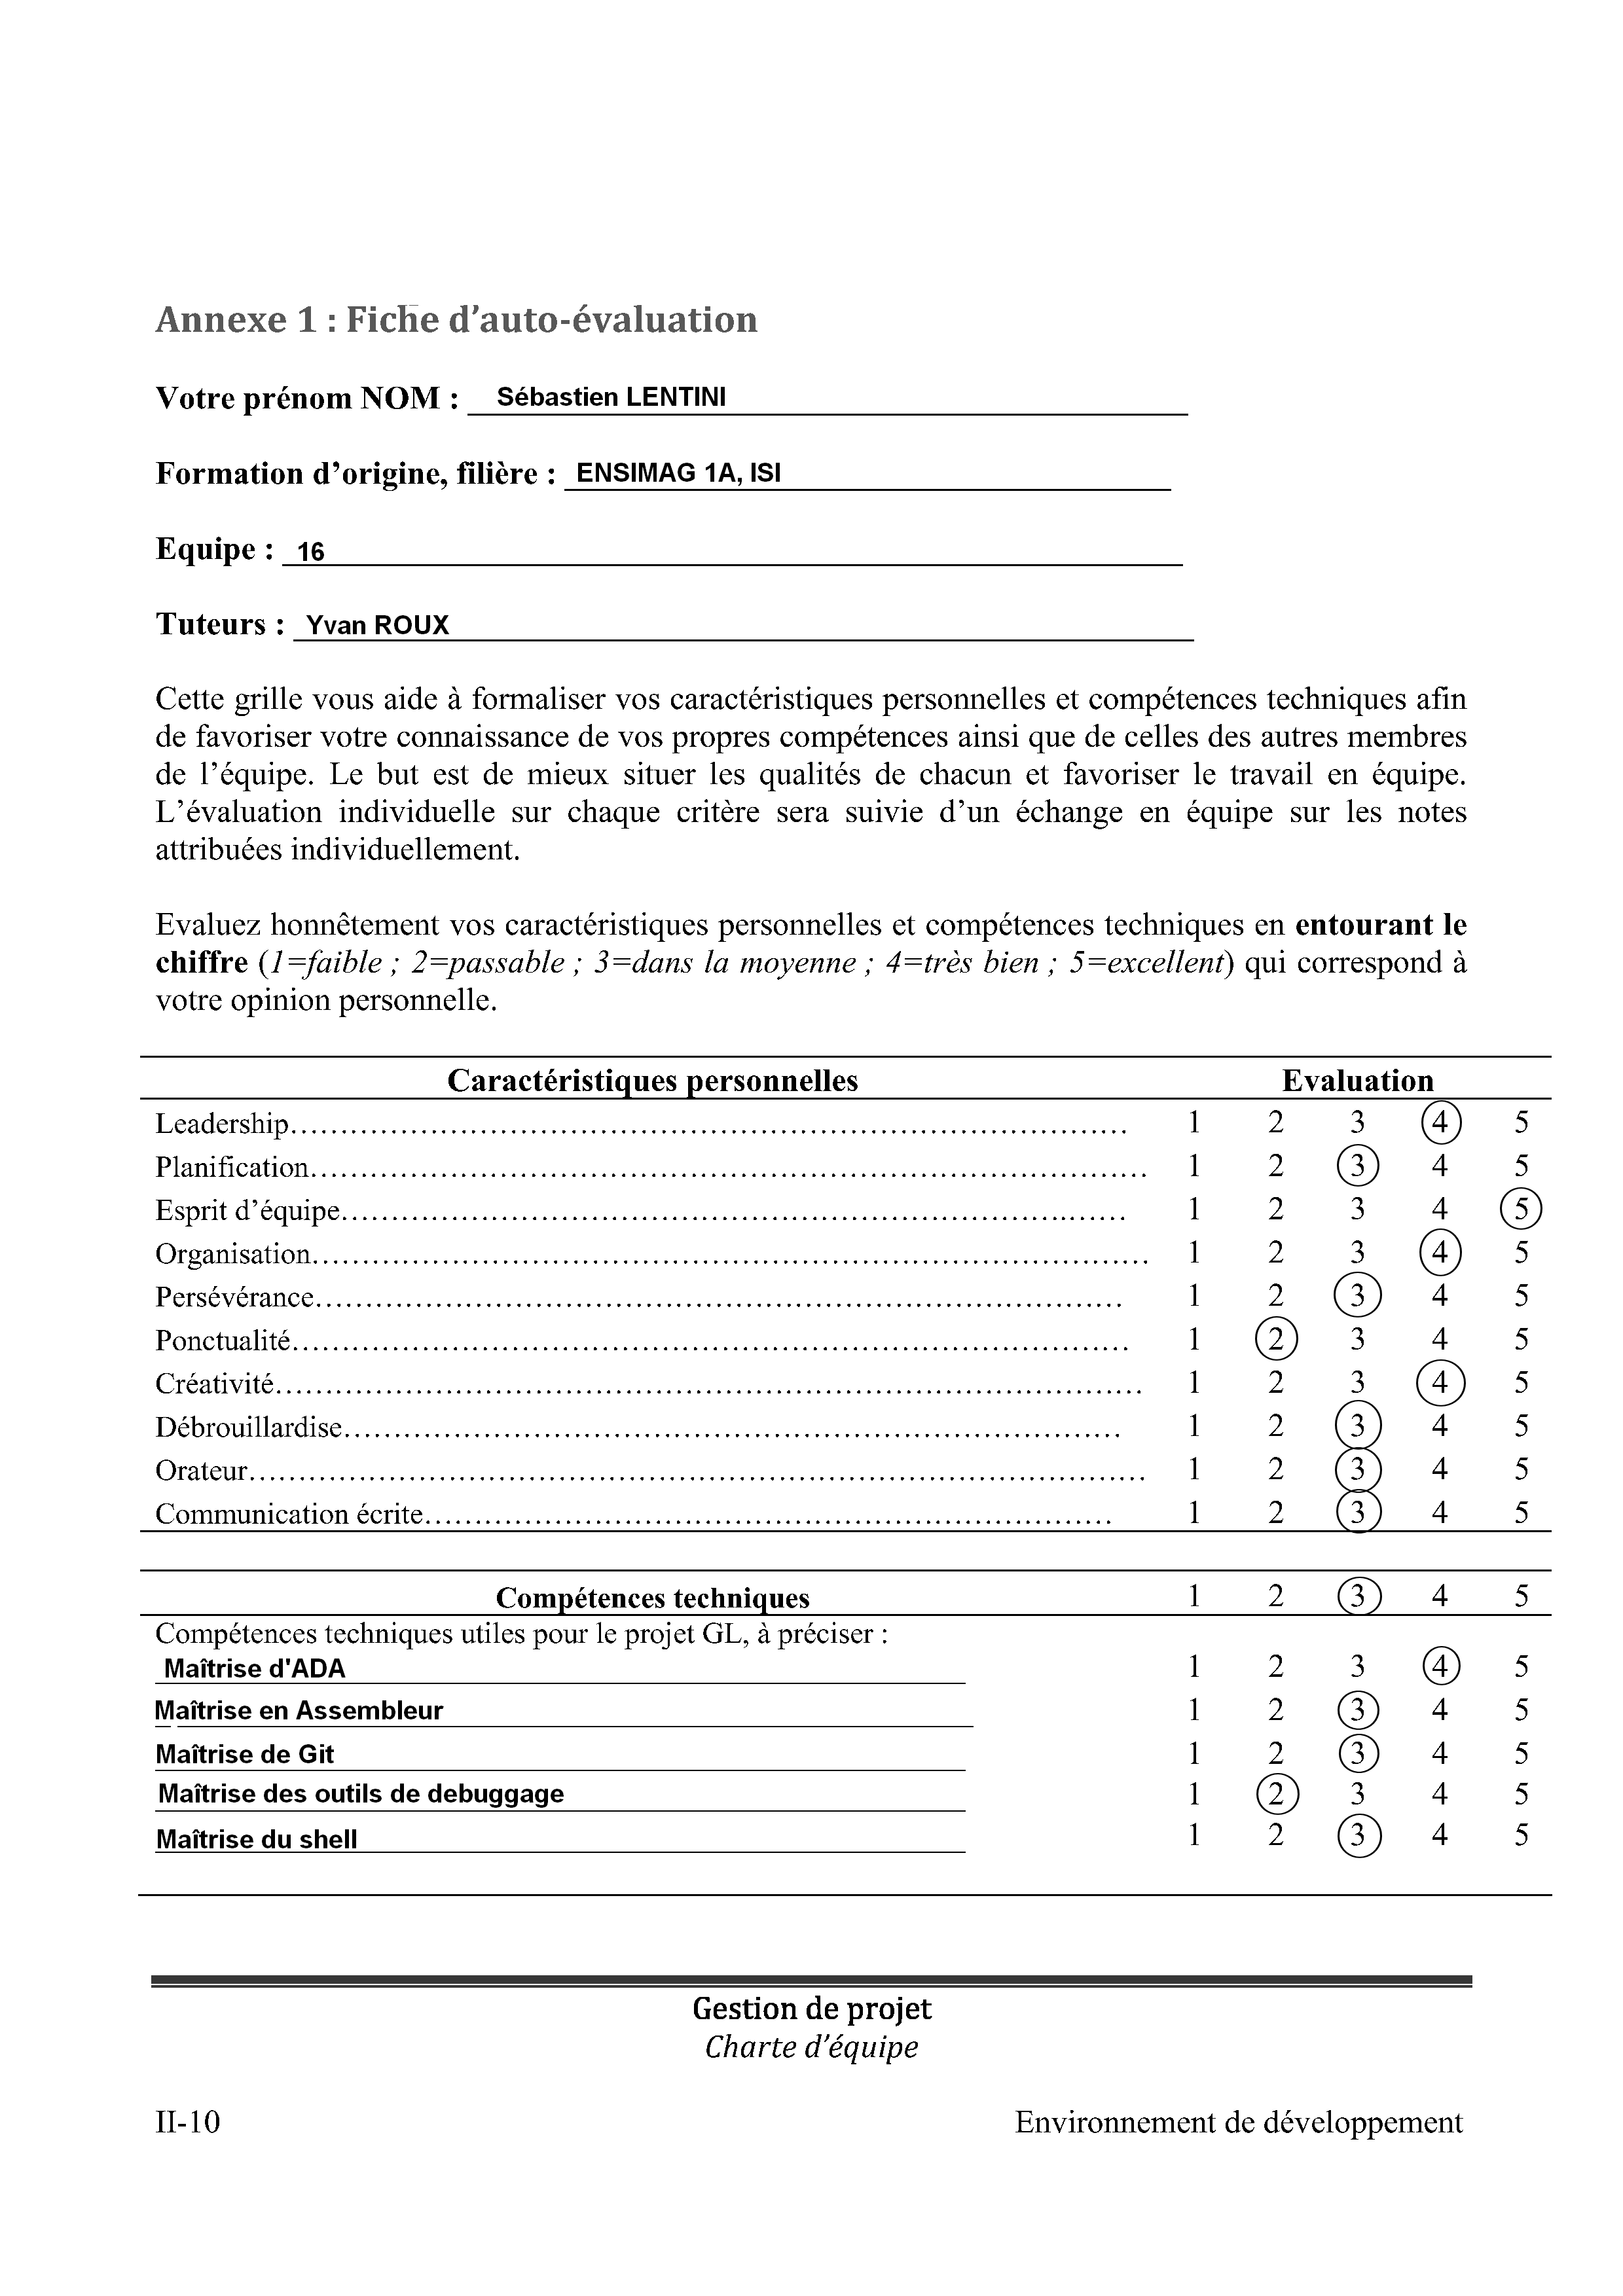
\includegraphics[scale=0.9]{auto-eval_Sebastien.png}
\newpage
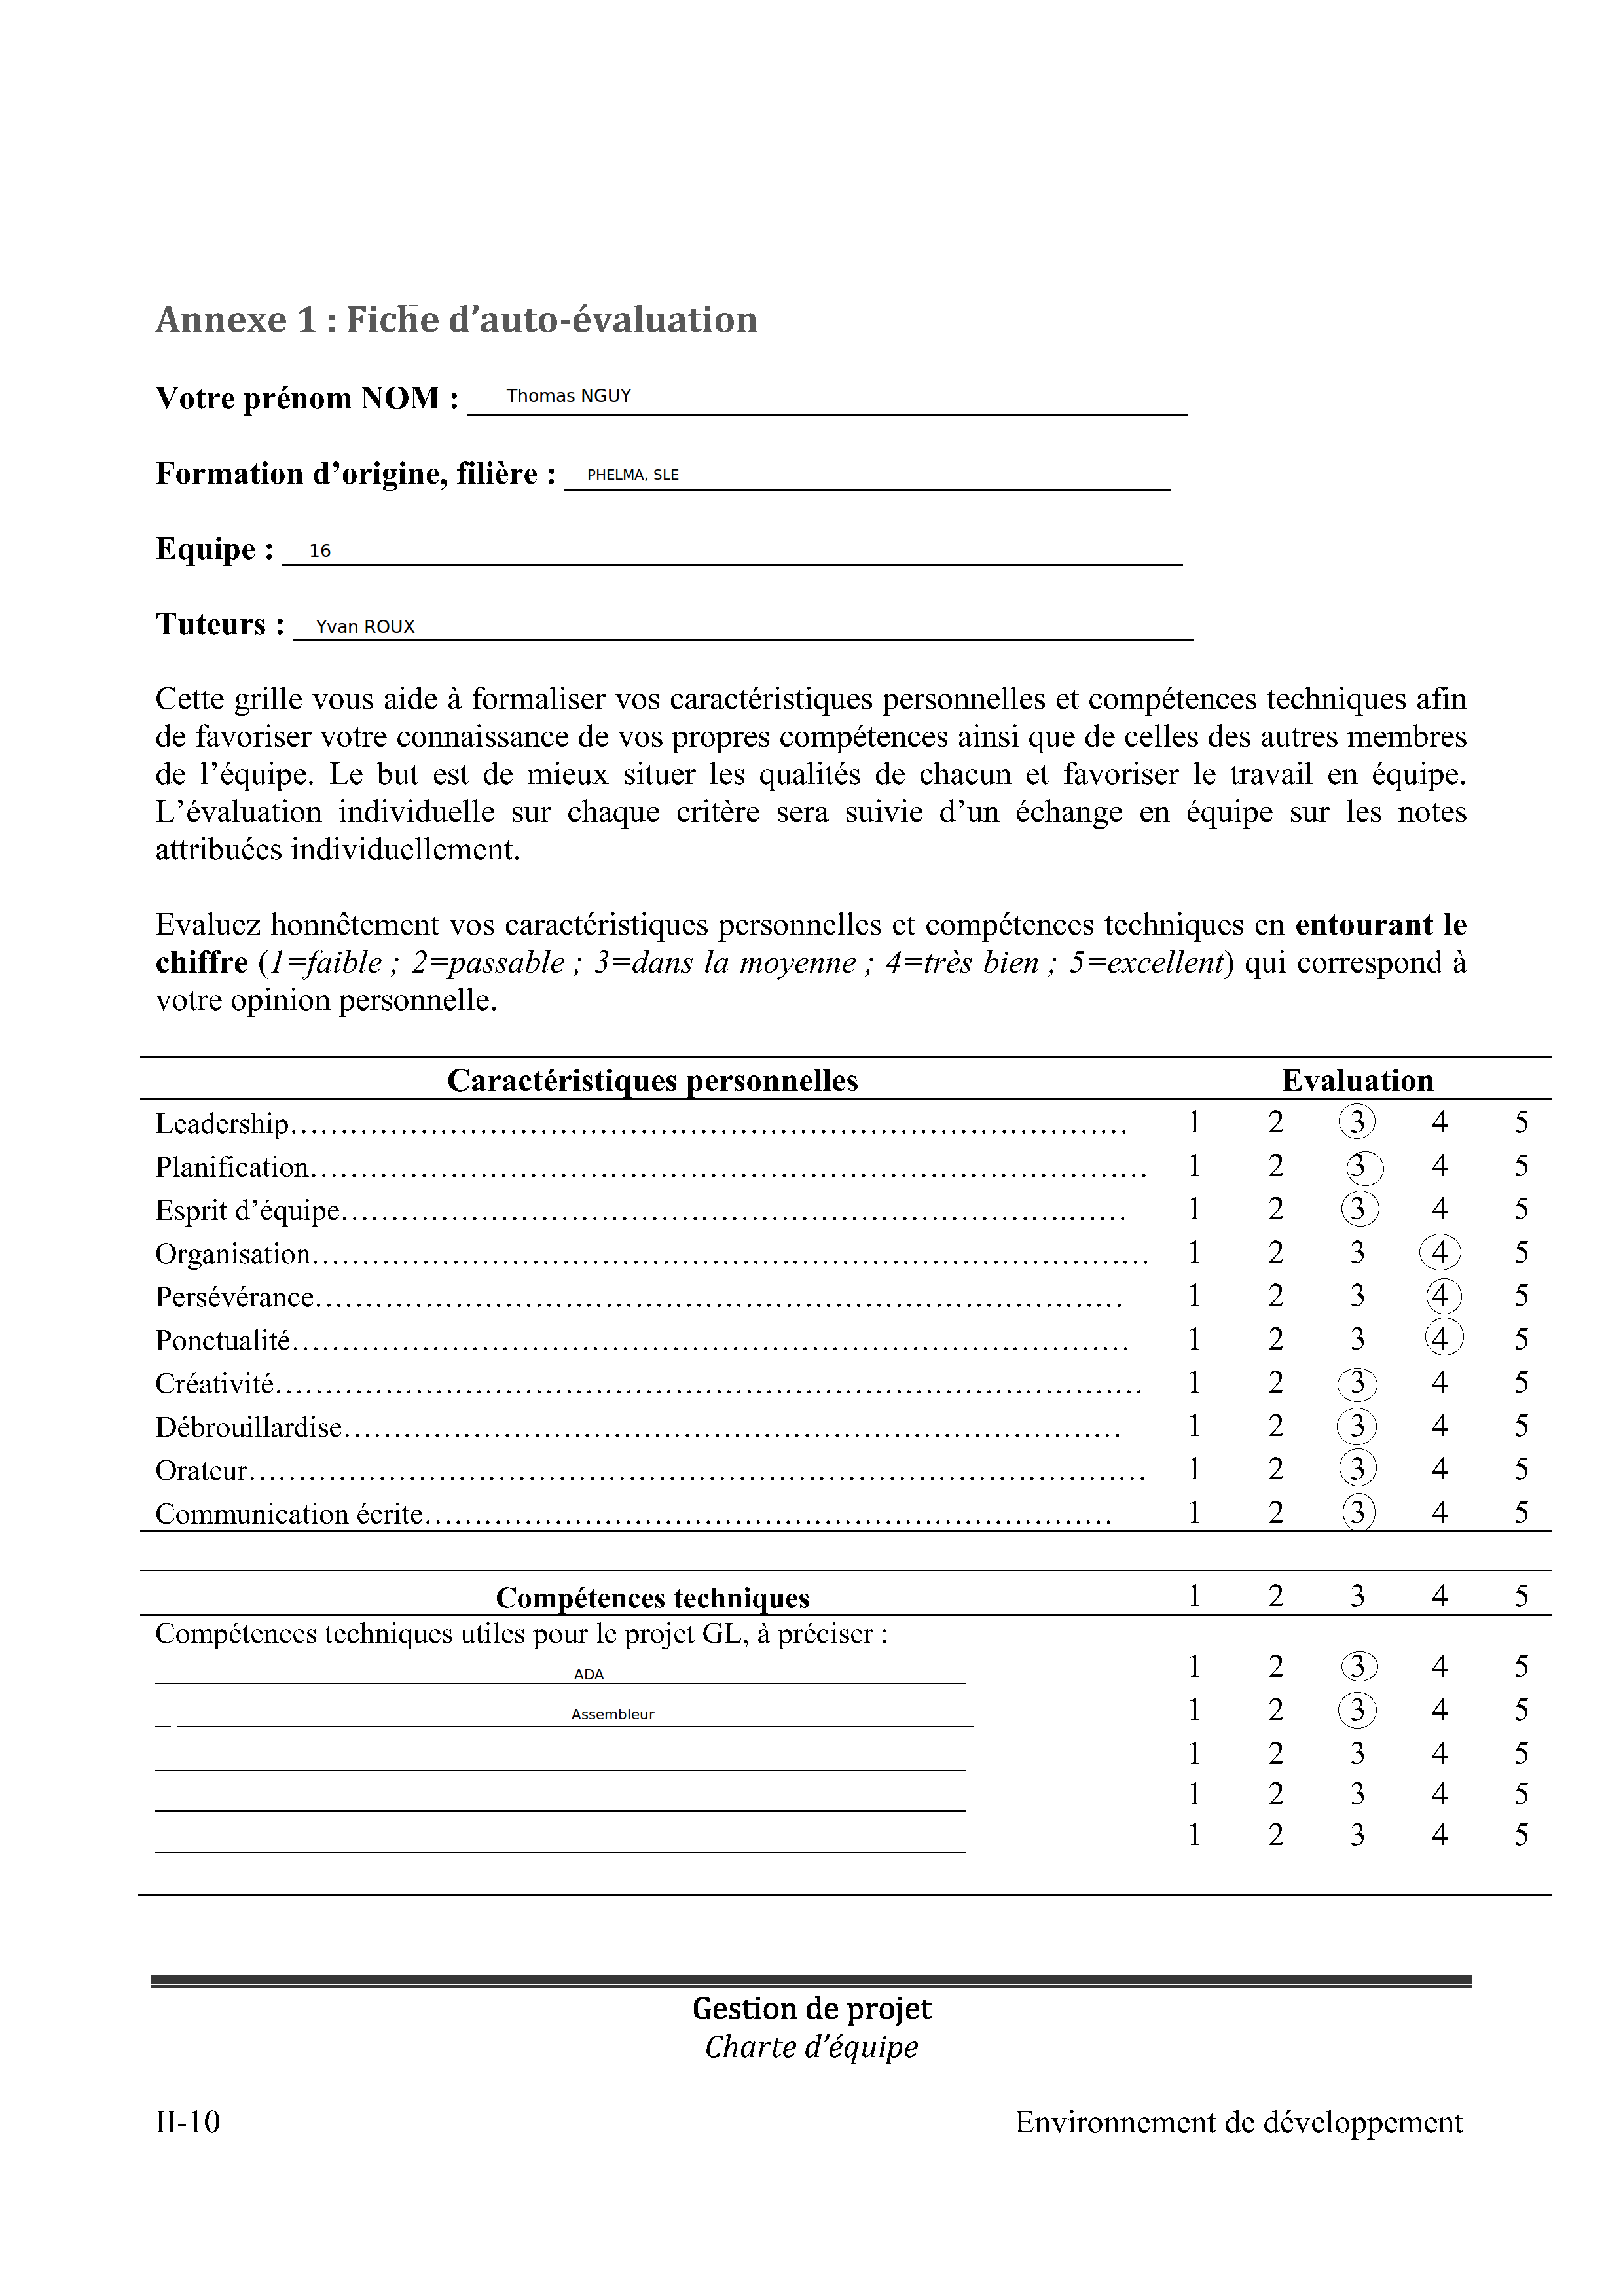
\includegraphics[scale=0.2]{auto-eval_Thomas.png}

\end{document}
\end{document}
